% Created 2019-06-27 Thu 18:54
% Intended LaTeX compiler: pdflatex
\documentclass[12pt, a4paper]{article}
\usepackage[utf8]{inputenc}
\usepackage[T1]{fontenc}
\usepackage{graphicx}
\usepackage{grffile}
\usepackage{longtable}
\usepackage{wrapfig}
\usepackage{rotating}
\usepackage[normalem]{ulem}
\usepackage{amsmath}
\usepackage{textcomp}
\usepackage{amssymb}
\usepackage{capt-of}
\usepackage{hyperref}
\usepackage[style=authoryear,natbib]{biblatex}
\setlength\bibitemsep{\baselineskip}
\addbibresource{/Users/guilhermesalome/Dropbox/references.bib}
\usepackage[T1]{fontenc}
\usepackage{lmodern}
\usepackage{amsmath}
\usepackage{mathtools}
\usepackage{multirow}
\usepackage{booktabs}
\usepackage{bbm}
\usepackage{dsfont}
\usepackage[]{algorithm2e}
\newcommand\numberthis{\addtocounter{equation}{1}\tag{\theequation}}
\newcommand{\E}[1]{\mathbb{E}{\left[#1\right]}}
\newcommand{\EQ}[1]{\mathbb{E}_t^{\mathbb{Q}}{\left[#1\right]}}
\newcommand{\EP}[1]{\mathbb{E}_t^{\mathbb{P}}{\left[#1\right]}}
\newcommand{\e}[1]{\text{e}^{#1}}
\newcommand{\abs}[1]{\left\vert{#1}\right\vert}
\newcommand{\dis}{\overset{d}{\sim}}
\newcommand{\Var}[1]{\mathrm{Var}\left(#1\right)}
\newcommand{\Corr}[1]{\mathrm{Corr}\left(#1\right)}
\newcommand{\Normal}[1]{\mathcal{N}\left(0, #1\right)}
\newcommand{\Max}[1]{\text{max}\left\{#1\right\}}
\newcommand{\Set}[1]{\left\{#1\right\}}
\renewcommand{\ln}[1]{\text{ln}\left(#1\right)}
\DeclareMathOperator*{\argmin}{\arg\!\min}
\DeclareMathOperator*{\argmax}{\arg\!\max}
\DeclarePairedDelimiter\ceil{\lceil}{\rceil}
\DeclarePairedDelimiter\floor{\lfloor}{\rfloor}
\newcommand{\Poisson}[1]{\text{Poisson}\left(#1\right)}
\newcommand{\Uniform}[1]{\text{Unif}#1}
\newcommand{\Cov}[1]{\mathrm{Cov}\left(#1\right)}
\newtheorem{problem}{Problem}
\usepackage[hang,small,bf]{caption}
\usepackage[margin=1in]{geometry}
\usepackage{mathtools}
\usepackage{xcolor}
\usepackage{resizegather}
\usepackage{multirow}
\definecolor{darkgreen}{rgb}{0.1, 0.6, 0.1}
\usepackage{float}
\usepackage{fancyhdr}
\pagestyle{fancy}
\fancypagestyle{plain}{}
\fancyhf{}
\rfoot{Page \thepage}
\usepackage{ifthen}
\rhead{\ifthenelse{\value{page}=1}{Guilherme Salom\'{e}}{Summer \the\year}}
\lhead{\ifthenelse{\value{page}=1}{Econ890-01 Matlab}{Econ890-01 Matlab}}
\usepackage[numbered,framed]{matlab-prettifier}
\usepackage{listings}
\date{}
\title{Measuring and Improving Code Performance}
\hypersetup{
 pdfauthor={Guilherme Salomé},
 pdftitle={Measuring and Improving Code Performance},
 pdfkeywords={},
 pdfsubject={},
 pdfcreator={Emacs 26.1 (Org mode 9.2.1)},
 pdflang={English}}
\begin{document}

\maketitle
\section{Measuring Performance}
\label{sec:org66d4946}
Matlab offers two main tools for measuring the performance of code and finding out its bottlenecks.
The first are the timing functions, which can be used to measure how long pieces of code and functions take to run.
The second is the profiling tool of Matlab, which can measure the performance of large pieces of code (several functions) and displays results in a nice interface.
\subsection{Timing}
\label{sec:org79e4a32}
We can time pieces of code with the functions \href{https://www.mathworks.com/help/matlab/ref/tic.html?s\_tid=doc\_ta}{\texttt{tic}} and \href{https://www.mathworks.com/help/matlab/ref/toc.html?s\_tid=doc\_ta}{\texttt{toc}}.
When \texttt{tic} is executed, it starts an internal stopwatch and returns a number (optional) representing the time when \texttt{tic} was executed.
The function \texttt{toc} displays how much time has elapsed in seconds since the function \texttt{tic} was executed.
Subsequent calls to \texttt{toc} display how much time has elapsed since the first \texttt{tic} has been executed.
We can start a new timer by calling \texttt{tic} again.

We can use \texttt{tic} and \texttt{toc} to time pieces of code.
\lstset{language=matlab,label= ,caption= ,captionpos=b,firstnumber=1,numbers=left,style=Matlab-editor}
\begin{lstlisting}
% measure how long it takes to execute the code below
% start timer
tic
n = 10000;
a = rand(n, n);
b = rand(n, 1);
a*b;
toc

% we can store the time in a variable
t = toc;

% measure time depending on size of matrix
n_values = 1:500:10000;
t = zeros(length(n_values), 1);
for i = 1:length(n_values)
    tic;
    n = n_values(i);
    a = rand(n, n);
    b = rand(n, 1);
    a*b;
    t(i) = toc;
end
plot(n_values, t)
\end{lstlisting}
We can create more than one timer by saving the output of \texttt{tic}, which can then be passed to \texttt{toc} to measure the time difference with respect to the respective \texttt{tic}.
\lstset{language=matlab,label= ,caption= ,captionpos=b,firstnumber=1,numbers=left,style=Matlab-editor}
\begin{lstlisting}
total_time = tic;
repetitions = 100;
times = zeros(length(repetitions), 1);
for rep = 1:repetitions
    t = tic;
    % do computation
    mean(randn(10000000, 1));
    % store time
    times(rep) = toc(t);
end
% average time
disp(sprintf('Average time: %.2f seconds (%d repetitions)', ...
     mean(times), length(times)));
% total time
disp(sprintf('Total time: %.2f seconds', toc(total_time)));
\end{lstlisting}
The functions \texttt{tic} and \texttt{toc} are good to time small pieces of code, but to get a more precise time estimation it is necessary to re-run the same code several times and average the \texttt{tic} and \texttt{toc} results.

A more rigorous timing measure can be obtained with the function \href{https://www.mathworks.com/help/matlab/ref/timeit.html}{\texttt{timeit}}.
We can use \texttt{timeit} to measure the typical time it takes to run a function.
Given a function, \texttt{timeit} runs it several times and reports the median time it takes to complete its execution.

Create a test function:
\lstset{language=matlab,label= ,caption= ,captionpos=b,firstnumber=1,numbers=left,style=Matlab-editor}
\begin{lstlisting}
% test_timeit.m
function [a, b] = test_timeit(X)
beta = rand(size(X, 2), 1);
a = X*beta;
if nargout > 1
    b = exp(a);
end
\end{lstlisting}

Use \texttt{timeit} to time the execution of the function:
\lstset{language=matlab,label= ,caption= ,captionpos=b,firstnumber=1,numbers=left,style=Matlab-editor}
\begin{lstlisting}
% specify the input to test_timeit
X = rand(5000);
timeit(@() test_timeit(X))
% specify how many outputs the function being timed should return
timeit(@() test_timeit(X), 2)
\end{lstlisting}
\subsection{Profiling}
\label{sec:org655ece7}
The command \href{https://www.mathworks.com/help/matlab/ref/profile.html}{\texttt{profile}} can be used to profile large pieces of code.
We can start the profiler by executing \texttt{profile on}.
Then, any code that we run afterwards will be automatically timed.
We can then call \texttt{profile viewer} to stop the profiler and see the results in a new window.
Let's first create a test code:
\lstset{language=matlab,label= ,caption= ,captionpos=b,firstnumber=1,numbers=left,style=Matlab-editor}
\begin{lstlisting}
% test_profiler.m
clear all
clc
% Load stock data
data = readmatrix('AAPL.csv');
% Compute intraday log-returns
prices = reshape(data(:, 3), 78, []);
returns = diff(log(prices));
% Compute realized variance
RV = sum(returns.^2);
% Generate bootstrap samples to compute confidence interval
total_samples = 10000;
RVs = zeros(total_samples, length(RV));
pbar = waitbar(0, 'Bootstrapping');     % progress bar
for i = 1:total_samples
    % generate bootstrap indices
    indices = unidrnd(size(returns, 1), size(returns, 1), 1);
    % bootstrap sample of the returns
    returns_sample = returns(indices, :);
    % compute statistic for each day
    RVs(i, :)  = sum(returns_sample.^2);
    % generate progress bar
    waitbar(i/total_samples, pbar);
end
close(pbar);
% Compute confidence interval
CI = quantile(RVs, [0.005 0.995])';
% Generate timestamps for plotting
dates = data(1:78:end, 1);
years = floor(dates./10000);
months = floor((dates - years.*10^4)./100);
days = floor(dates - years.*10^4 - months.*10^2);
sdates = datenum(years, months, days);
% Plot realized variance with correct x-ticks
plot(sdates, RV, 'k');
datetick('x', 'yyyy');
grid on;
% Shade confidence interval region
hold on;
f = fill([sdates; flip(sdates)], [CI(:, 1); flip(CI(:, 2))], 'k');
f.FaceAlpha = 0.2;
f.EdgeAlpha = 0;
\end{lstlisting}

Now, we can use the profiler to analyze the code for bottlenecks.
Clear the workspace before running the profiler.
\lstset{language=matlab,label= ,caption= ,captionpos=b,firstnumber=1,numbers=left,style=Matlab-editor}
\begin{lstlisting}
clear all
profile on
test_profiler
profile viewer
\end{lstlisting}

The command \texttt{profile viewer} displays the window shown in Figure \ref{fig:org8fa407f}.

\begin{figure}[H]
\centering
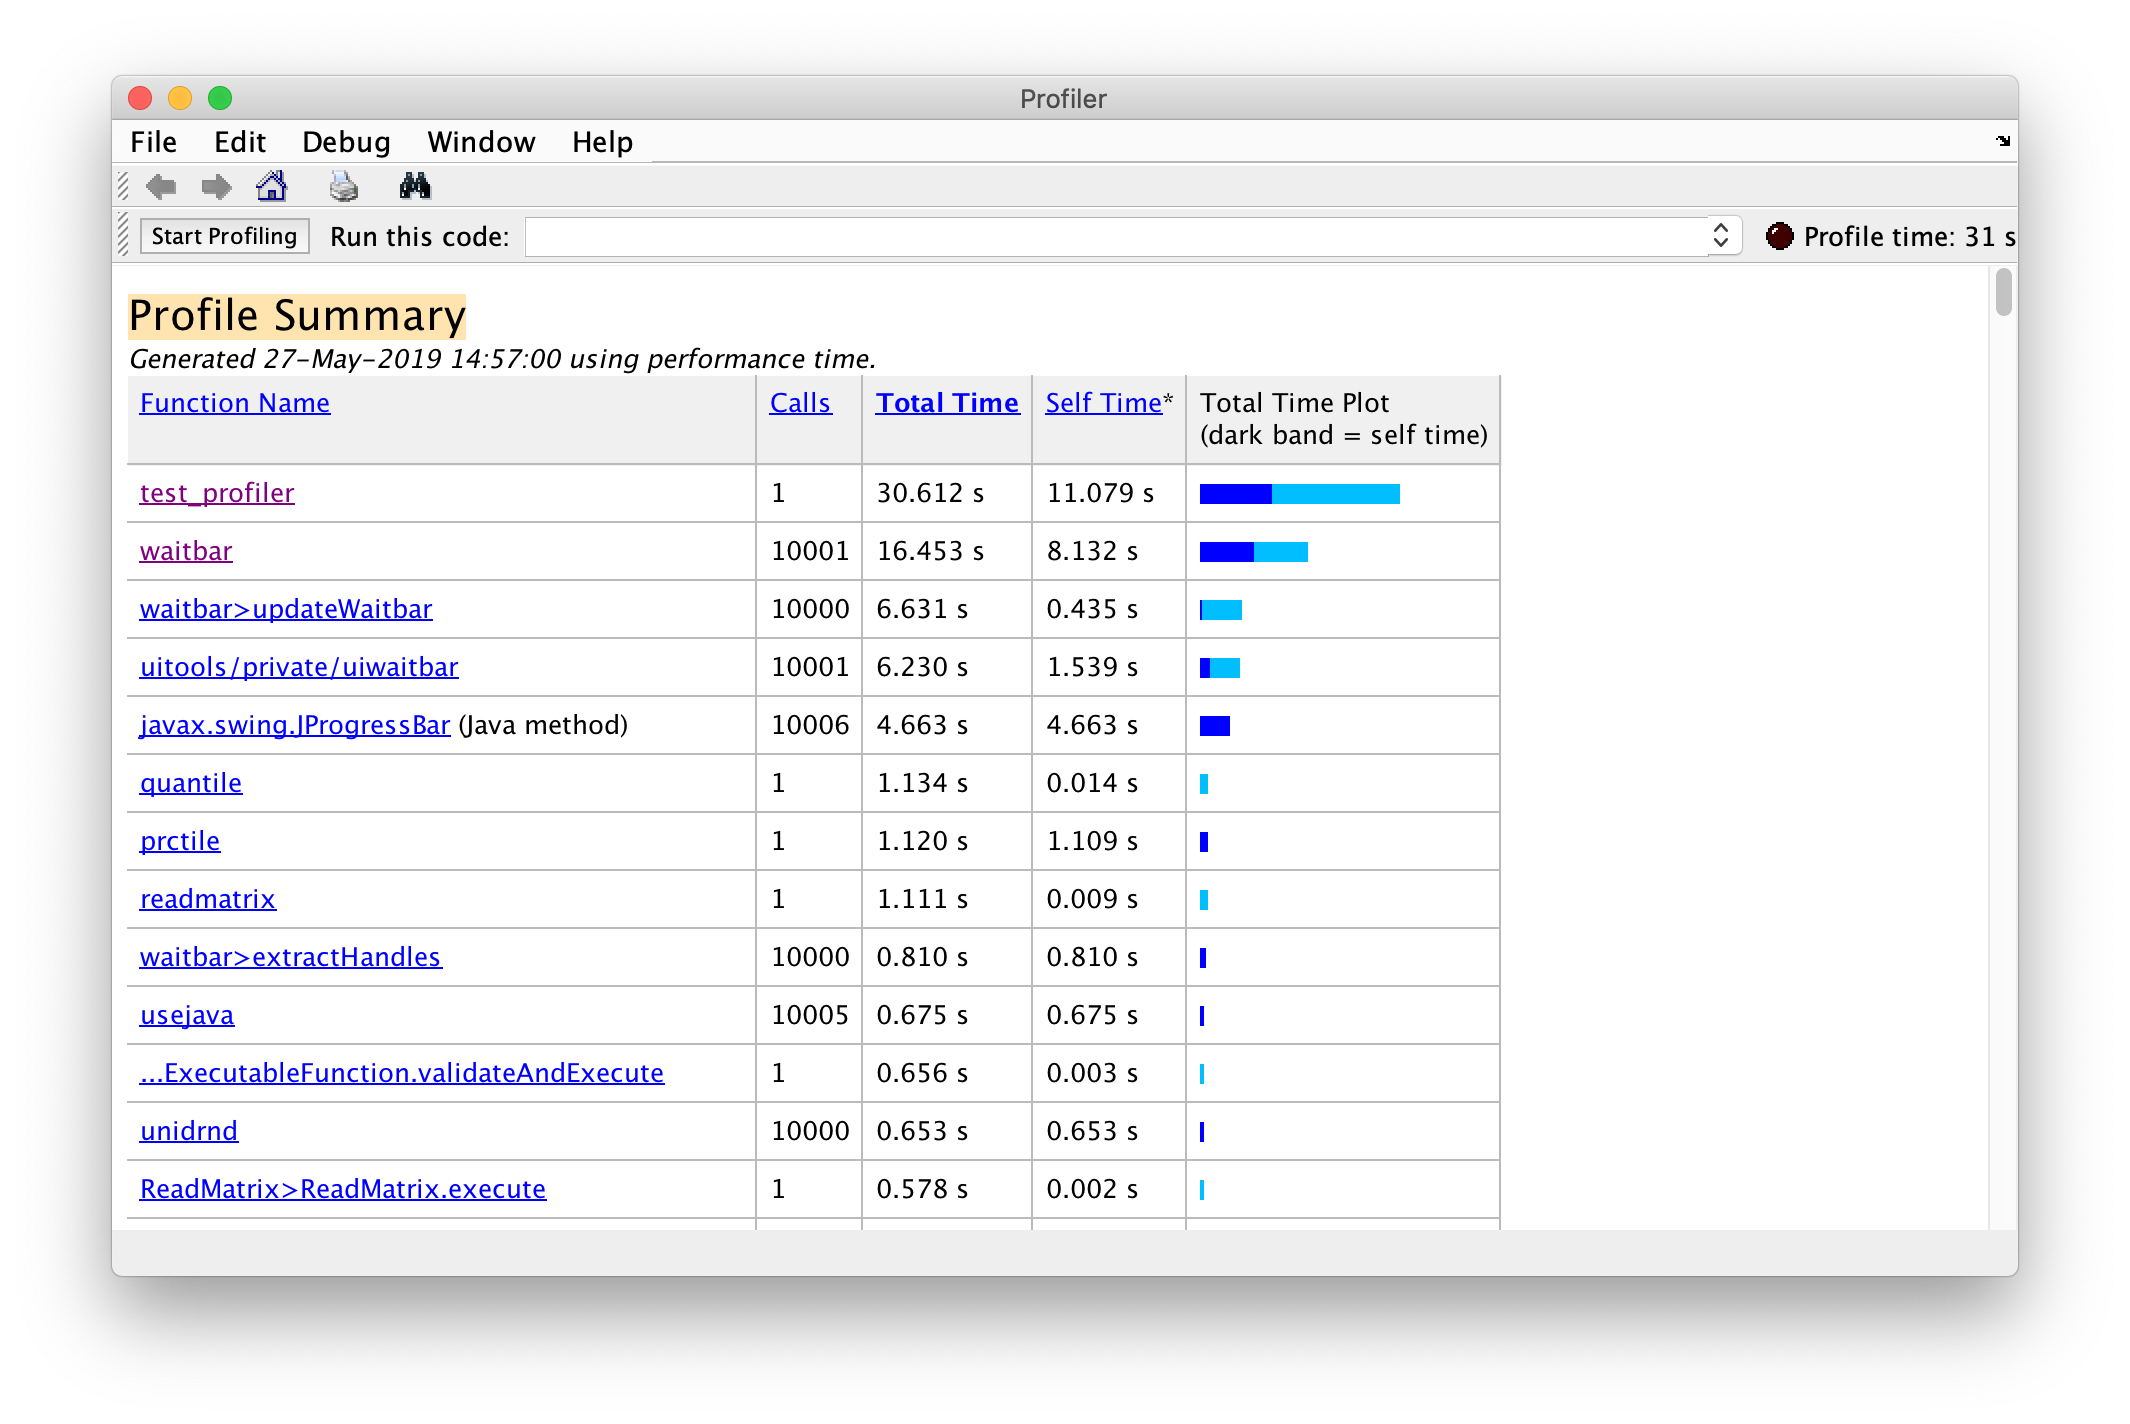
\includegraphics[width=8cm]{/Users/guilhermesalome/Teaching/Duke/Econ890 Matlab - 2019/supporting/matlab_profile_summary.png}
\caption{\label{fig:org8fa407f}
Profile Summary Window.}
\end{figure}

The profiler window shows all functions called while the profiler was on.
The functions are sorted by total executing time.
You can click on each function to see a more detailed break down of the execution.
Click on the \texttt{test\_profiler} function, and you should see a window similar to what Figure \ref{fig:orge708250} displays.

\begin{figure}[H]
\centering
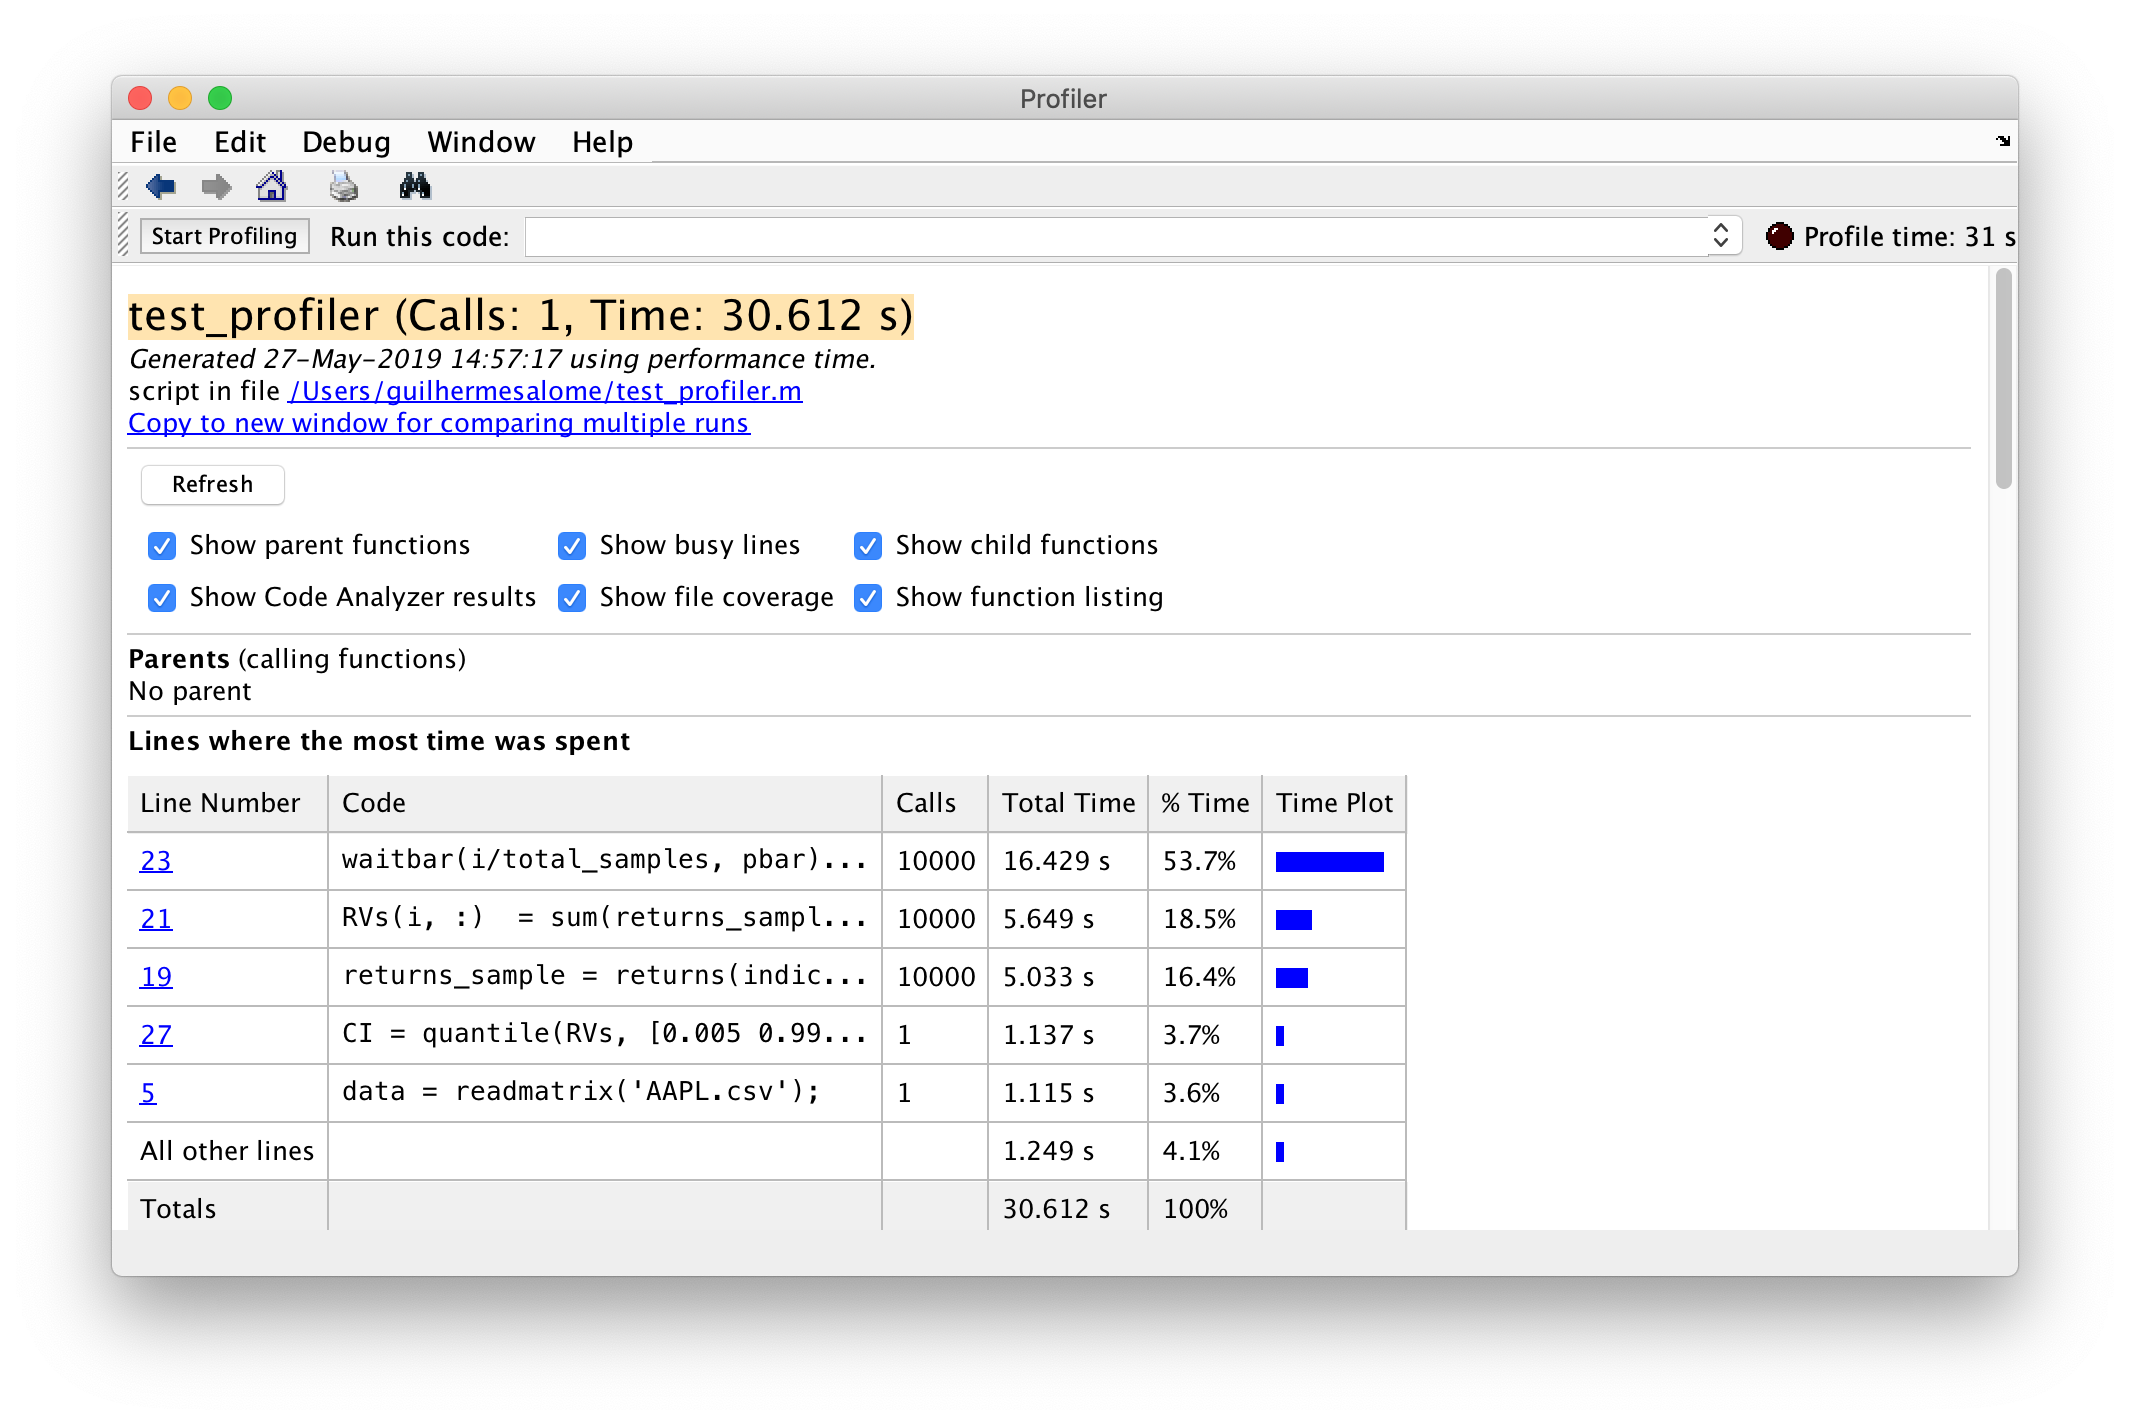
\includegraphics[width=8cm]{/Users/guilhermesalome/Teaching/Duke/Econ890 Matlab - 2019/supporting/matlab_profiler_detail.png}
\caption{\label{fig:orge708250}
Profiler Detail Window.}
\end{figure}

We see that the \texttt{test\_profiler} function took around 30 seconds to finish running.
The window also shows the lines where most of the time was spent.
We see that out of the 30 seconds, almost 5 seconds were spent on generating bootstrap samples from the original returns.
That line was executed 10000 times.
You can click on the line number to see the code around it.
Click on the button for line \texttt{19}.
You should see a window similar to what is displayed in Figure \ref{fig:org2723441}.

\begin{figure}[H]
\centering
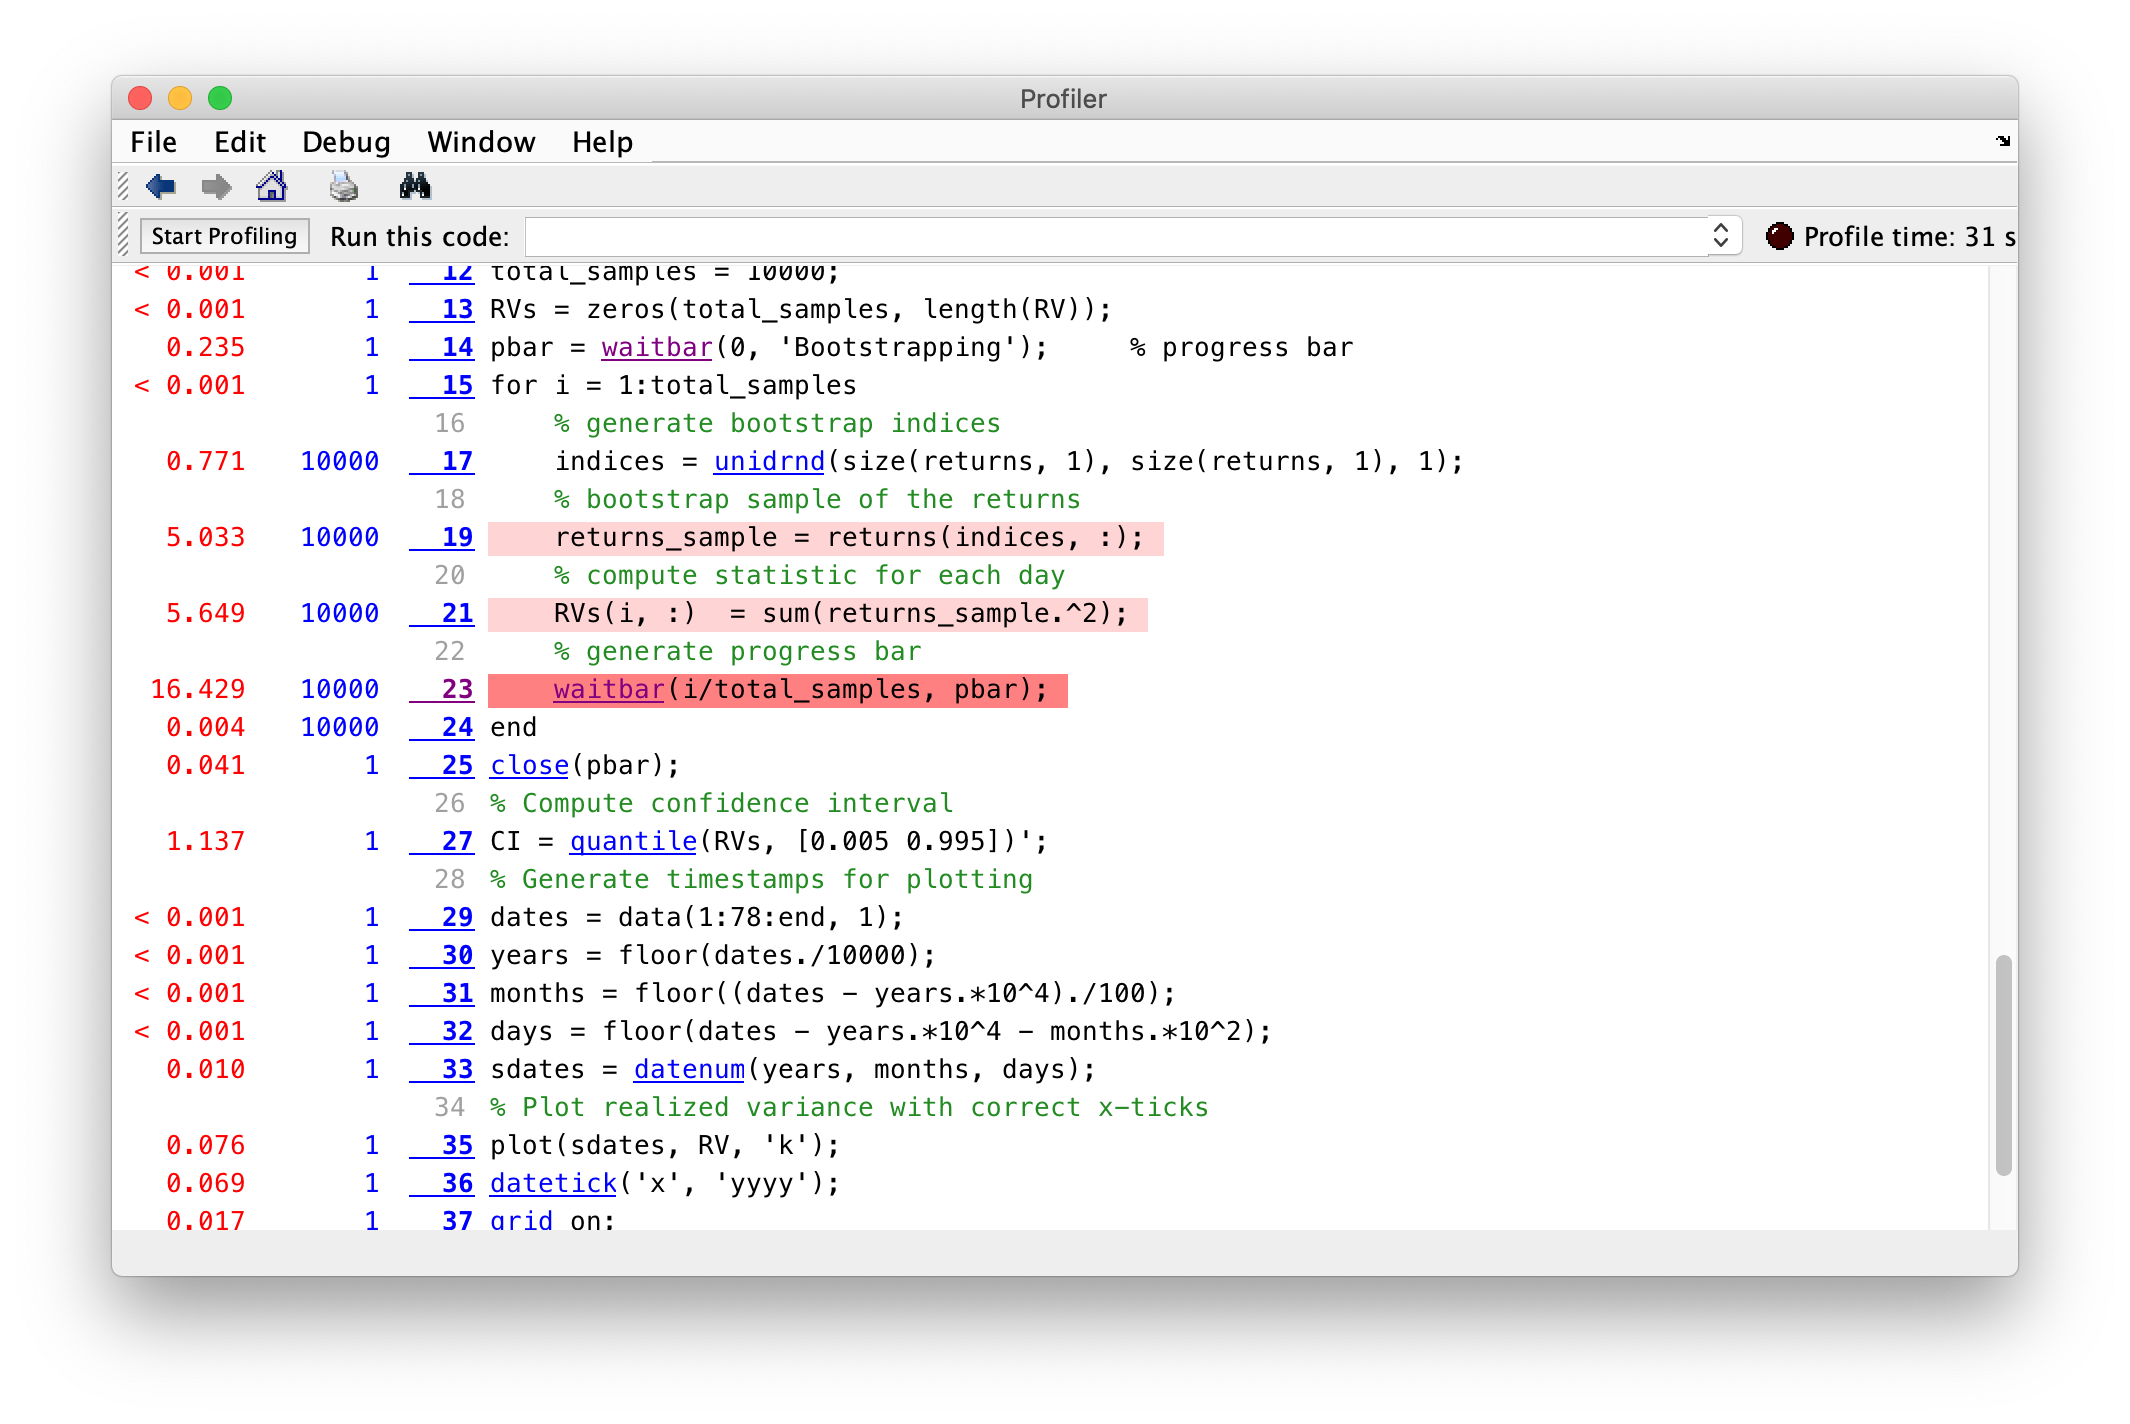
\includegraphics[width=8cm]{/Users/guilhermesalome/Teaching/Duke/Econ890 Matlab - 2019/supporting/matlab_profiler_code_time.png}
\caption{\label{fig:org2723441}
Profiler Line by Line Timing.}
\end{figure}

The lines displayed in darker red are the ones that take longer to execute.
Lines 19 and 21 take about the same time to execute, while updating the progress bar takes the longest.
We can use this information to identify lines that are inefficient, update the code and test again.

We can save the profiler results by executing the command \href{https://www.mathworks.com/help/matlab/ref/profsave.html?s\_tid=doc\_ta}{\texttt{profsave}}, which stores the results in a folder named \texttt{profile\_results}.
The file \texttt{file0.html} contains the same information as the profiler summary window, displayed in Figure \ref{fig:org8fa407f}.

Using the profiler is useful when working with a data set that is large.
The idea is to use a small subset of the data to develop your code, then time it to see how long it takes.
Then, you extrapolate how much time it would take to run your code on the entire data set.
If the total time is acceptable then you are done.
However, if it is not, then you should profile the code and see where you could improve it before running on the entire data set.
\section{Efficiency Tips}
\label{sec:org6768268}
We will now cover some general tips for efficiency when coding.
Let's use the functions \texttt{tic} and \texttt{toc} to check the difference in execution time.

Avoid creating temporary objects:
\lstset{language=matlab,label= ,caption= ,captionpos=b,firstnumber=1,numbers=left,style=Matlab-editor}
\begin{lstlisting}
times = zeros(1000, 1);
for i = 1:1000
    tic
    %% Code to time
    A = 2*randn(10000, 100);
    B = A.^2;
    % store time
    times(i) = toc;
end
% report median
disp(sprintf('Median execution time: %.4f seconds', median(times)));

times = zeros(1000, 1);
for i = 1:1000
    tic
    %% Code to time
    B = (2*randn(10000, 100)).^2;
    % store time
    times(i) = toc;
end
% report median
disp(sprintf('Median execution time: %.4f seconds', median(times)));
\end{lstlisting}
The object stored in \texttt{A} is temporary, created at the beginning of each loop, then used to compute \texttt{B}, and then reassigned when a new loop starts.
We can avoid creating and deleting \texttt{A} by moving the \texttt{randn} command into \texttt{B}.

Pre-allocate matrices whenever possible.
\lstset{language=matlab,label= ,caption= ,captionpos=b,firstnumber=1,numbers=left,style=Matlab-editor}
\begin{lstlisting}
%% Append to vector
tic
a = [];
for j = 1:10000
    a = vertcat(a, randn(1));
end
disp(sprintf('Time: %.4f seconds', toc));
%% Pre-allocate and then modify vector
tic
a = zeros(10000, 1);
for j = 1:10000
    a(j) = randn(1);
end
disp(sprintf('Time: %.4f seconds', toc));
\end{lstlisting}
Creating a matrix and then extending it is slower than pre-allocating the matrix.
Extending the matrix means Matlab has to allocate more and more memory at each loop, recreating the vector \texttt{a} at each iteration.
This reduces the efficiency of the code and makes it slower.
Pre-allocating the matrix allows for a single block of memory to be allocated to the vector \texttt{a}.

Use sparse matrices to save memory when dealing with a large number of zeros.
\lstset{language=matlab,label= ,caption= ,captionpos=b,firstnumber=1,numbers=left,style=Matlab-editor}
\begin{lstlisting}
A = eye(10000);                         % not sparse
B = sparse(eye(10000));                 % sparse
whos A B;
\end{lstlisting}
Sparse arrays only stores the nonzero elements in memory.
It is possible to visualize the sparsity of a matrix with the function \href{https://www.mathworks.com/help/matlab/ref/spy.html?s\_tid=doc\_ta}{\texttt{spy}}.

Vectorize operations if possible:
\lstset{language=matlab,label= ,caption= ,captionpos=b,firstnumber=1,numbers=left,style=Matlab-editor}
\begin{lstlisting}
m_size = 1000000;
x = randn(m_size, 1);
y = rand(m_size, 1);
%% Not vectorized
z = zeros(m_size, 1);
tic
for i = 1:m_size
    z(i) = x(i)*y(i);
end
disp(sprintf('Time: %.4f seconds', toc));
%% Vectorized
clear z
tic
z = x.*y;
disp(sprintf('Time: %.4f seconds', toc));
\end{lstlisting}
A vectorized operation can run faster than a for-loop if it uses a built-in function.
It is also more self-documenting than a for-loop and often leads to fewer lines of code.
\section{Generating and Using C Code with Matlab}
\label{sec:org2beb8b0}
We can execute code written in C, C++ or Fortran with Matlab.
To do so, we need to create a binary file named \texttt{MEX}, which can then be called in Matlab as a regular function.
To create \texttt{MEX} files, we will use a Matlab tool that can convert Matlab code to some other language.
For this section you will need to install \href{https://www.mathworks.com/help/coder/index.html?s\_tid=CRUX\_lftnav}{Matlab Coder} (or learn how to code in \href{https://en.wikipedia.org/wiki/C\_(programming\_language)}{C} or \href{https://en.wikipedia.org/wiki/C\%2B\%2B}{C++}).
You can also execute \texttt{coder} on Matlab to get a prompt to install it.

We will learn how to generate the \texttt{MEX} files with an example.
Write the following function:
\lstset{language=matlab,label= ,caption= ,captionpos=b,firstnumber=1,numbers=left,style=Matlab-editor}
\begin{lstlisting}
% euclidean_dist.m
function [distances, point_min, point_max] = euclidean_dist(x,points)
% Compute Euclidean norm between x and the points
distances = sum((x-points).^2).^0.5;
% Obtain points that maximize and minimize the distance
[~, id_min] = min(distances);
[~, id_max] = max(distances);
% Save these points
point_min = points(:, id_min);
point_max = points(:, id_max);
end
\end{lstlisting}
This functions takes a column vector \texttt{x}, and a matrix containing multiple column vectors \texttt{points}, then computes the Euclidean distance between \texttt{x} and the other points.
The functions has three outputs, the distance between all points, the vector closest to \texttt{x} and the vector farthest from \texttt{x}.

Now, we need to use Matlab's Code Analyzer.
To do so, add the comment \texttt{\%\#codegen} right after the definition of the function \texttt{euclidean\_dist}:
\lstset{language=matlab,label= ,caption= ,captionpos=b,firstnumber=1,numbers=left,style=Matlab-editor}
\begin{lstlisting}
function [distances, point_min, point_max] = euclidean_dist(x,points) %#codegen
\end{lstlisting}
This will trigger the Code Analyzer to check for any issues that could prevent the Matlab code from being converted to C/C++.
If there are no errors, a green square will appear on the upper right-hand side of the Editor window.
If there are errors, then the lines with issues will be underlined in red.
You can hover the mouse on top of the line to see a message explaining the issue and how to fix it.
Most of the features of the programming language are supported by the converter, but some are not.
For a full list of the supported and unsupported features, see \href{https://www.mathworks.com/help/simulink/ug/matlab-language-features-supported-for-code-generation.html}{this reference page}.

Figure \ref{fig:orgd88ae96} displays the results of the Code Analyzer for the function \texttt{euclidean\_dist}.

\begin{figure}[H]
\centering
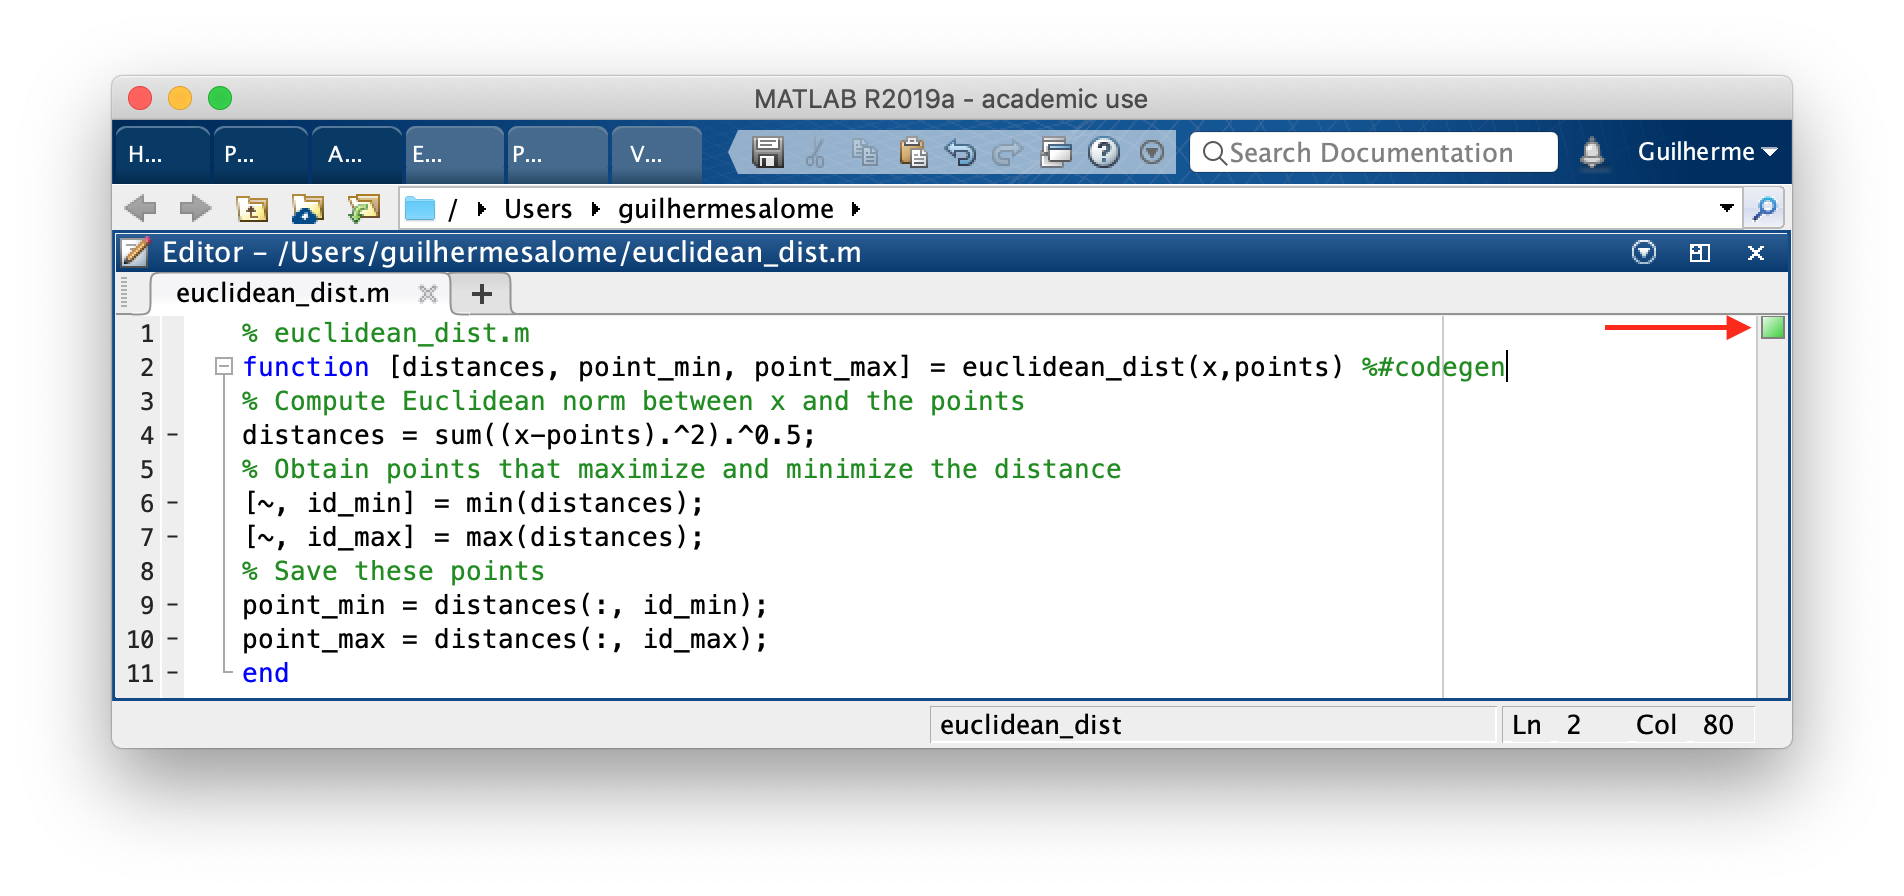
\includegraphics[width=8cm]{/Users/guilhermesalome/Teaching/Duke/Econ890 Matlab - 2019/supporting/matlab_code_analyzer_output.png}
\caption{\label{fig:orgd88ae96}
Code Analyzer Without Errors.}
\end{figure}

Now, we will use the function \href{https://www.mathworks.com/help/coder/ref/coder.screener.html?s\_tid=doc\_ta}{\texttt{coder.screener}} to call the \href{https://www.mathworks.com/help/coder/ug/code-generation-readiness-tool.html}{Code Generation Readiness Tool}.
This tool also checks for possible issues that can arise when generating the C/C++ code.
\lstset{language=matlab,label= ,caption= ,captionpos=b,firstnumber=1,numbers=left,style=Matlab-editor}
\begin{lstlisting}
coder.screener('euclidean_dist')
\end{lstlisting}

Figure \ref{fig:org61fcbd4} shows the output of the code above.
It indicates the function we created should not lead to issues when being converted to C/C++ code.
\begin{figure}[H]
\centering
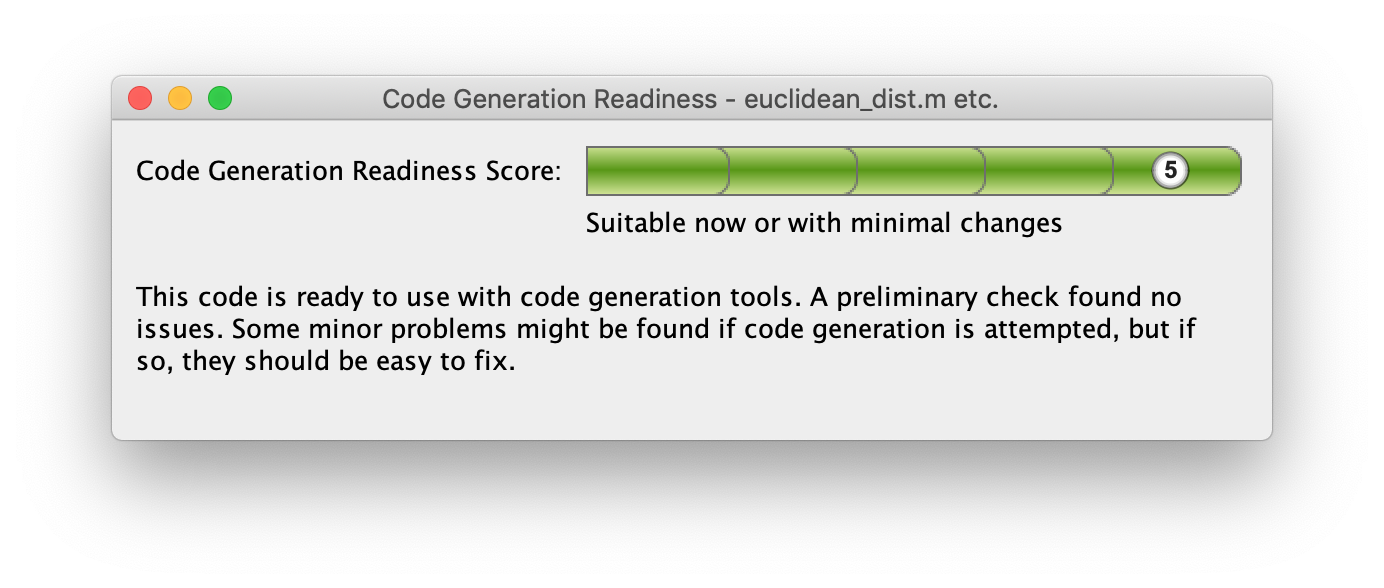
\includegraphics[width=8cm]{/Users/guilhermesalome/Teaching/Duke/Econ890 Matlab - 2019/supporting/matlab_code_generation_readiness.png}
\caption{\label{fig:org61fcbd4}
Output of Code Generation Readiness Tool.}
\end{figure}

We can now generate the \texttt{MEX} file with the \href{https://www.mathworks.com/help/coder/ref/codegen.html}{\texttt{codegen}} command.
The \texttt{MEX} file is based on C code, which is statically typed.
This means we need to define the type (class) and size of the inputs to the function when generating the lower-level code.
We start with the case where the size of the inputs is fixed.

\subsection{Fixed-Size Inputs}
\label{sec:org048ea1c}
The type and size of inputs can be inferred when generating the lower-level code by giving an example to the command \texttt{codegen}.
\lstset{language=matlab,label= ,caption= ,captionpos=b,firstnumber=1,numbers=left,style=Matlab-editor}
\begin{lstlisting}
% create example for codegen
x = [1; 2; 3];                          % size 3 x 1
points = rand(3, 10);                   % size 3 x 10
\end{lstlisting}
To create the \texttt{MEX} file, we call \texttt{codegen} by passing it the name of the file we want to convert and the example inputs:
\lstset{language=matlab,label= ,caption= ,captionpos=b,firstnumber=1,numbers=left,style=Matlab-editor}
\begin{lstlisting}
codegen -report euclidean_dist.m -args {x, points}
\end{lstlisting}
The option \texttt{-report} generates a report that we can use to debug any issues that arise during the conversion.
After the \texttt{-report}, we have the file name, in this case \texttt{euclidean\_dist.m}, and then the option \texttt{-args} and a cell containing the example inputs.
The \texttt{codegen} command infers the type and size of the inputs from the type and size of \texttt{x} and \texttt{points}.

When we execute the code above you will see an error.
The error is depicted in Figure \ref{fig:org28ba2e1}.

\begin{figure}[H]
\centering
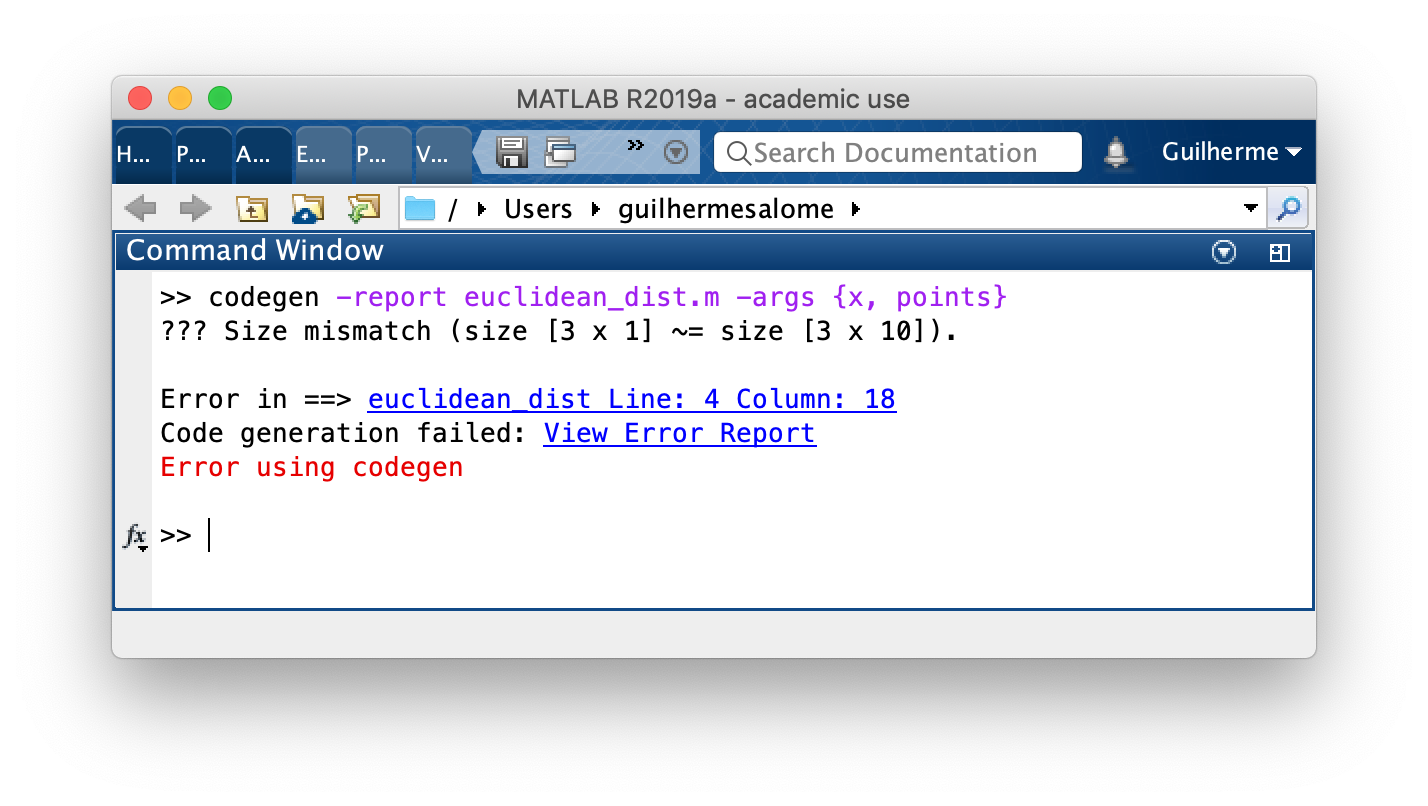
\includegraphics[width=8cm]{/Users/guilhermesalome/Teaching/Duke/Econ890 Matlab - 2019/supporting/matlab_codegen_error.png}
\caption{\label{fig:org28ba2e1}
Codegen Error.}
\end{figure}

The error says there is some type of mismatch in the code.
We can get more detail by clicking on \texttt{View Error Report}, which will open the window depicted in Figure \ref{fig:org32c0117}.

\begin{figure}[H]
\centering
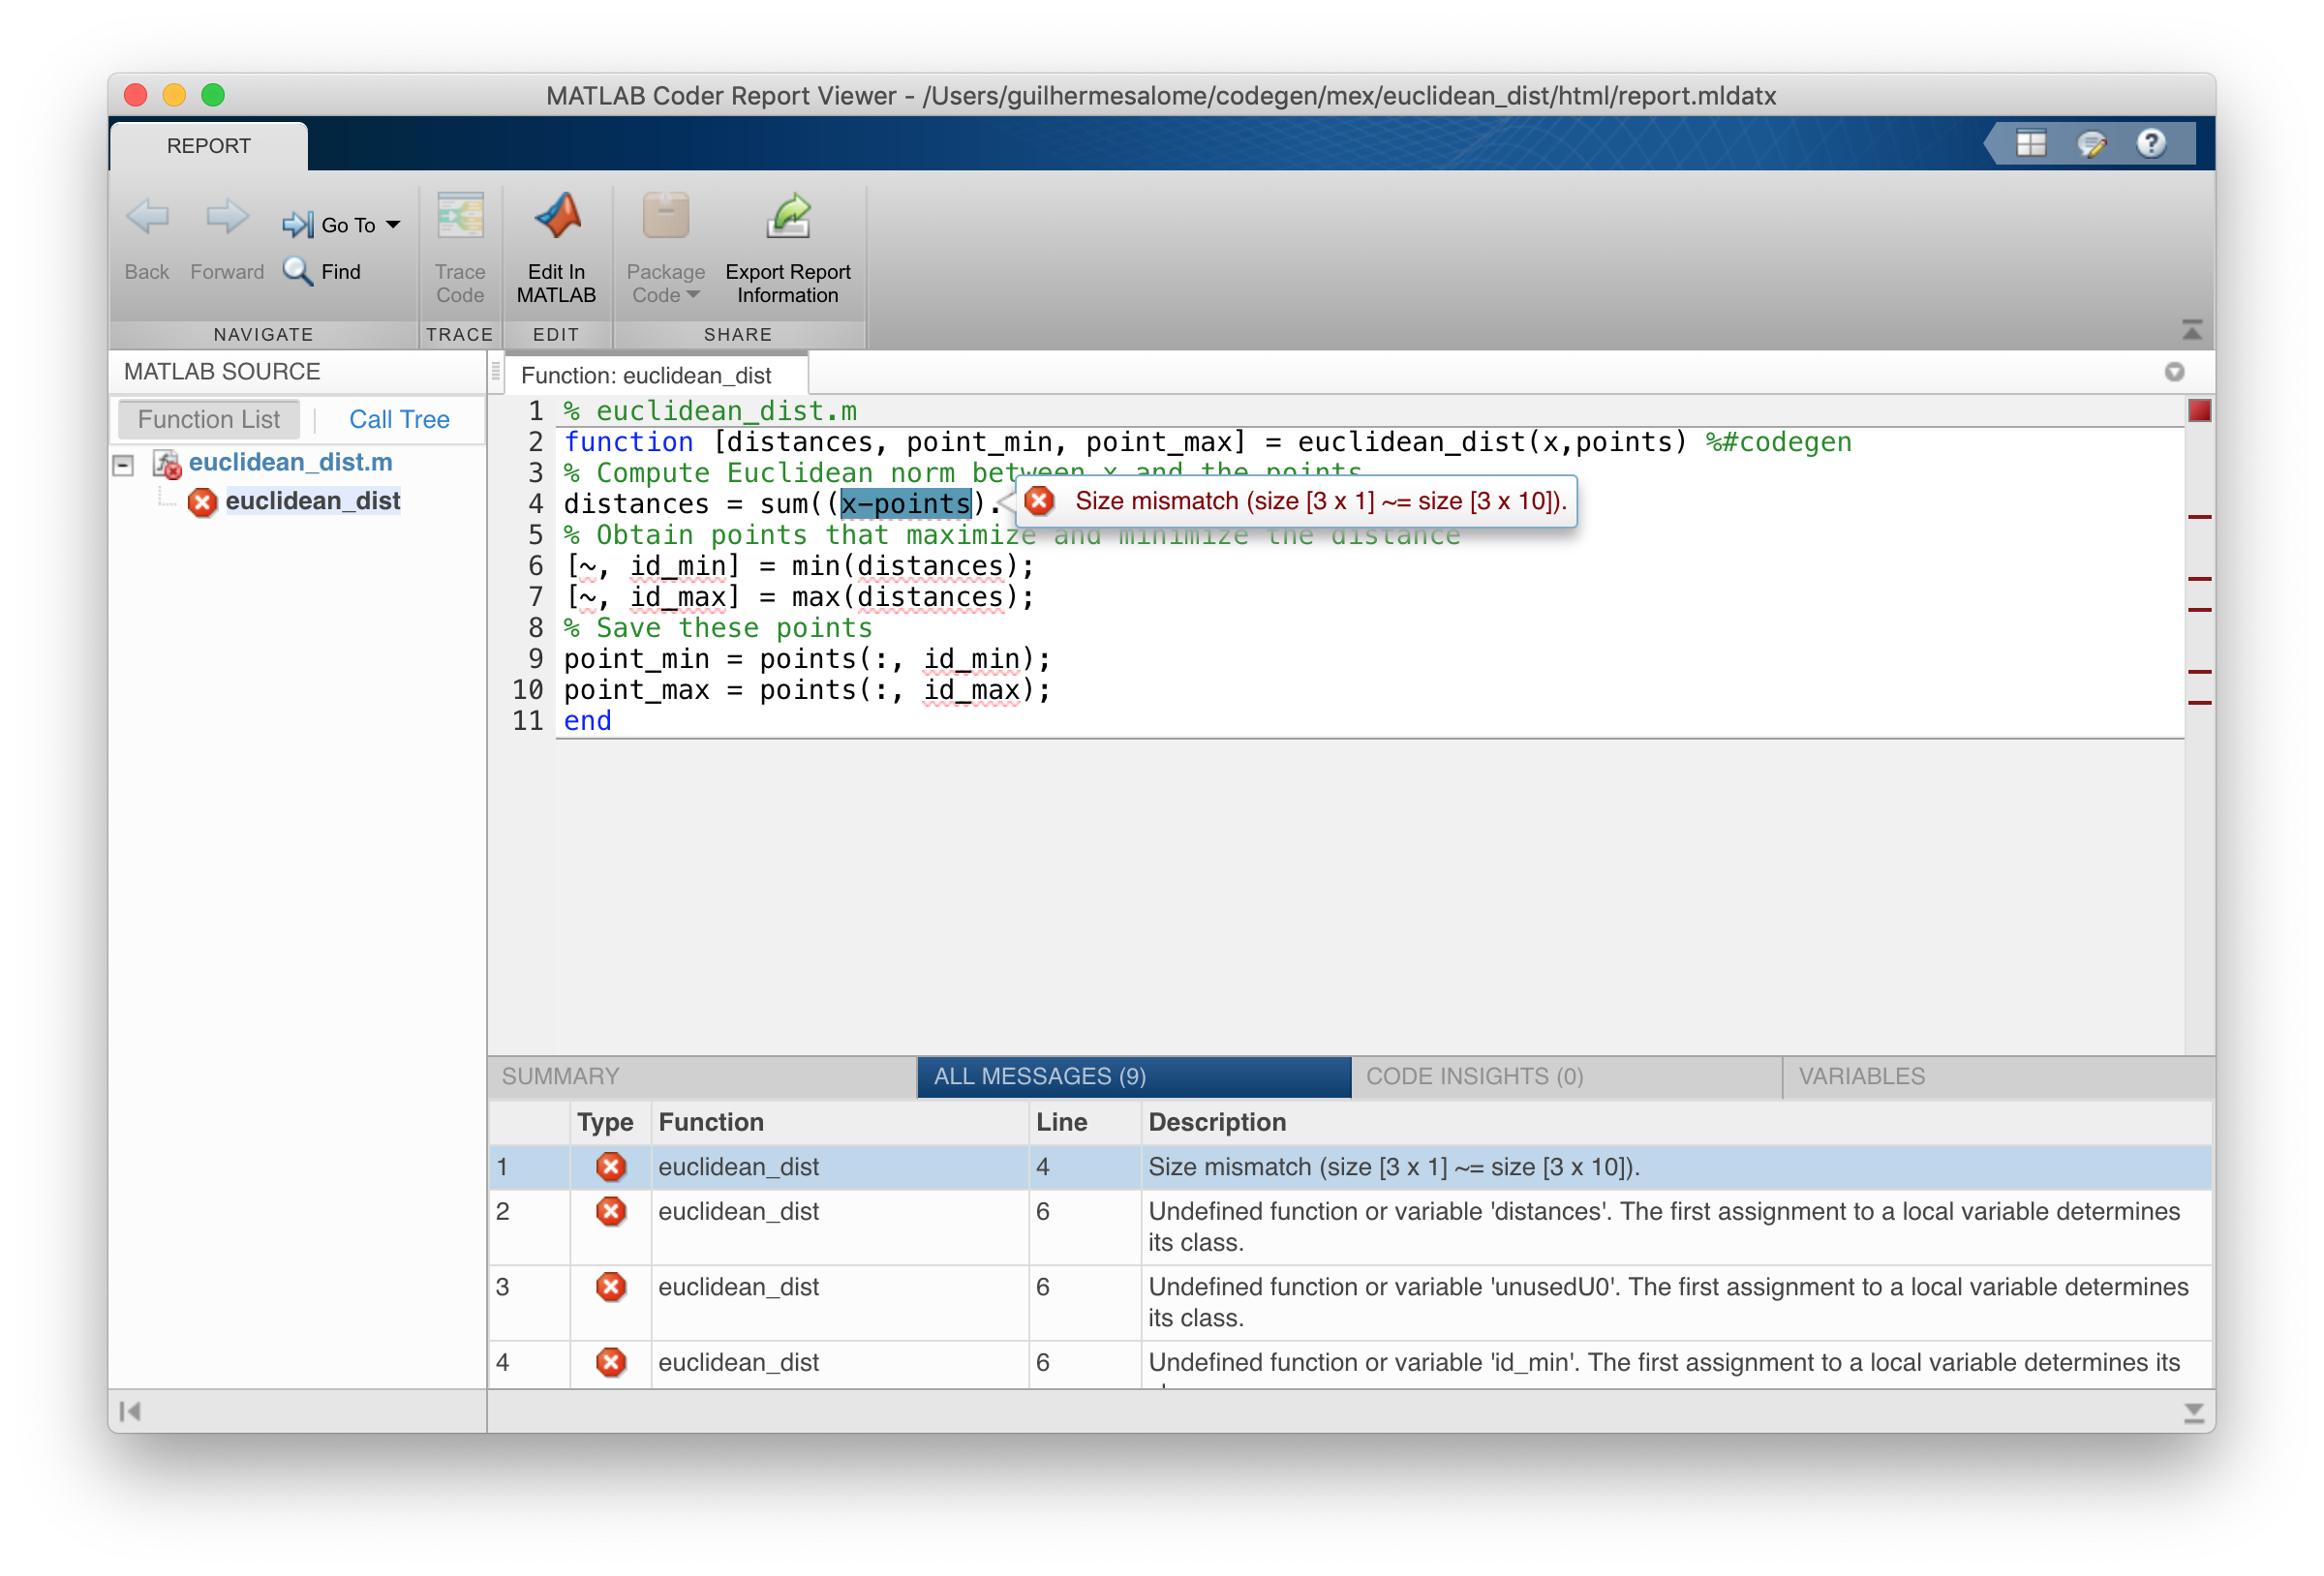
\includegraphics[width=8cm]{/Users/guilhermesalome/Teaching/Duke/Econ890 Matlab - 2019/supporting/matlab_codegen_report.png}
\caption{\label{fig:org32c0117}
Codegen Report and Error Message.}
\end{figure}

The error report shows that there is a mismatch in size between \texttt{x} and \texttt{points}.
It is not an issue in the Matlab code, because when we execute \texttt{x-points}, the vector \texttt{x} is broadcasted to have the same size of \texttt{points}.
However, it leads to an issue when converting the code to C.
We can fix it, by using \href{https://www.mathworks.com/help/matlab/ref/repmat.html?s\_tid=doc\_ta}{\texttt{repmat}} on the vector \texttt{x} to avoid the mismatch:
\lstset{language=matlab,label= ,caption= ,captionpos=b,firstnumber=1,numbers=left,style=Matlab-editor}
\begin{lstlisting}
% Modify the line:
distances = sum((x-points).^2).^0.5;
% To:
distances = sum((repmat(x, 1, size(points, 2))-points).^2).^0.5;
\end{lstlisting}

We can now compile the code by running:
\lstset{language=matlab,label= ,caption= ,captionpos=b,firstnumber=1,numbers=left,style=Matlab-editor}
\begin{lstlisting}
codegen -report euclidean_dist.m -args {x, points}
\end{lstlisting}

The code generation should complete successfully.
A file named \texttt{euclidean\_dist\_mex.mexmaci64} will be created.
This file contains the binaries that can be executed by Matlab as a regular function.
We can compare the time it takes to run the original function and the compiled function:
\lstset{language=matlab,label= ,caption= ,captionpos=b,firstnumber=1,numbers=left,style=Matlab-editor}
\begin{lstlisting}
% use timeit to compare execution time of the functions
sprintf('Original Function: %.6f seconds', timeit(@() euclidean_dist(x, points), 3))
sprintf('MEX Function: %.6f seconds', timeit(@() euclidean_dist_mex(x, points), 3))
\end{lstlisting}

In this case, there is little gain since vectorized and simple operations in Matlab are already very fast.
However, the gains in speed will increase when loops are involved.

Notice that if you try to execute \texttt{euclidean\_dist\_mex} with a vector \texttt{points} of a size different than the one specified, you will get an error.
\lstset{language=matlab,label= ,caption= ,captionpos=b,firstnumber=1,numbers=left,style=Matlab-editor}
\begin{lstlisting}
points = rand(3, 5);
euclidean_dist_mex(x, points)           % error
\end{lstlisting}

Next, we modify the \texttt{MEX} file to accept an input that can vary in size.
\subsection{Variable-Size Inputs}
\label{sec:org4955076}
To have the \texttt{MEX} function accept inputs of varied sizes, we use the function \href{https://www.mathworks.com/help/coder/ref/coder.typeof.html}{\texttt{coder.typeof}} to specify the size of the inputs.
The function \texttt{coder.typeof} takes three inputs:
\begin{enumerate}
\item An example for the input (like \texttt{x});
\item A vector that specifies an upper bound for each dimension of the input;
\item A vector that specified whether each dimension of the input is variable in size or fixed in size.
\end{enumerate}

Suppose we want to allow \texttt{x} to have up to 10 rows, but always one column.
And we want \texttt{points} to have up to 10 rows, and up to 10 columns.
\lstset{language=matlab,label= ,caption= ,captionpos=b,firstnumber=1,numbers=left,style=Matlab-editor}
\begin{lstlisting}
x = [1; 2; 3];
example_x = coder.typeof(x, [10 1], [1 0]);
% [10 1] specifies the upper bound for the dimensions of x
% [1 0] specifies that the size of the first dimension is variable,
% while the second is fixed
points = rand(3, 10);
example_points = coder.typeof(points, [10 10], [1 1]);
% [10 10] specifies the upper bound for the dimensions of the points
% [1 1] specifies that both dimensions are variable
\end{lstlisting}

We can now compile the code as before with \texttt{codegen}, and use \texttt{example\_x} and \texttt{example\_points} as the examples, instead of \texttt{x} and \texttt{points}:
\lstset{language=matlab,label= ,caption= ,captionpos=b,firstnumber=1,numbers=left,style=Matlab-editor}
\begin{lstlisting}
codegen -report euclidean_dist.m -args {example_x, example_points}
\end{lstlisting}

This will overwrite \texttt{euclidean\_dist\_mex} with the new version.
We can test it:
\lstset{language=matlab,label= ,caption= ,captionpos=b,firstnumber=1,numbers=left,style=Matlab-editor}
\begin{lstlisting}
x = rand(7, 1);
points = rand(7, 3);
euclidean_dist_mex(x, points)
\end{lstlisting}

We can further modify the code to allow \texttt{x} to have as many rows as we want, but always one column.
And \texttt{points} to have as many rows and columns as we want.
\lstset{language=matlab,label= ,caption= ,captionpos=b,firstnumber=1,numbers=left,style=Matlab-editor}
\begin{lstlisting}
example_x = coder.typeof(x, [Inf 1], [1 0]);
example_points = coder.typeof(points, [Inf Inf], [1 1]);
codegen -report euclidean_dist.m -args {example_x, example_points}
\end{lstlisting}

This will overwrite \texttt{euclidean\_dist\_mex} with the new version.
We can test it:
\lstset{language=matlab,label= ,caption= ,captionpos=b,firstnumber=1,numbers=left,style=Matlab-editor}
\begin{lstlisting}
x = rand(23, 1);
points = rand(23, 40);
euclidean_dist_mex(x, points)
\end{lstlisting}
\subsection{Generating C Code}
\label{sec:org2534229}
If you have a \href{https://www.mathworks.com/support/requirements/supported-compilers.html}{supported C compiler} installed on your machine, you can also generate the C code from the Matlab files.
You do so by adding the option \texttt{-config:lib} when calling \texttt{codegen}:
\lstset{language=matlab,label= ,caption= ,captionpos=b,firstnumber=1,numbers=left,style=Matlab-editor}
\begin{lstlisting}
codegen -d matlab_to_c -report euclidean_dist.m -args {example_x, example_points}
\end{lstlisting}
Notice the use of the option \texttt{-d matlab\_to\_c}, which stores the resulting files in the folder named \texttt{matlab\_to\_c}.
\subsection{Observations}
\label{sec:org835a41e}
The \texttt{MEX} files are platform specific, so if you compile a file in Windows, for example, then you will not be able to re-use it in Linux.
However, if you have the original \texttt{.m} file you can re-compile it again in a different platform.

It is not possible to generate \texttt{MEX} files from Matlab scripts, only for functions.
If you need to convert a script, then you must write it in a function format.

If you are often converting a file to \texttt{MEX}, it is good practice to create a build script that will do the conversion.
For example:
\lstset{language=matlab,label= ,caption= ,captionpos=b,firstnumber=1,numbers=left,style=Matlab-editor}
\begin{lstlisting}
% generate_mex_euclidean_dist.m
% Generates .mex file for: euclidean_dist.m
% Define inputs
example_x = coder.typeof(x, [Inf 1], [1 0]);
example_points = coder.typeof(points, [Inf Inf], [1 1]);
% Call codegen
codegen -report euclidean_dist.m -args {example_x, example_points}
\end{lstlisting}
Then, we can execute \texttt{generate\_mex\_euclidean\_dist} on Matlab to generate the \texttt{MEX} file.
\section{Parallelization}
\label{sec:org4d040ac}
We can speed up the execution of code in Matlab by taking advantage of the multiple cores available in modern computers.
Matlab offers a relatively easy way to make for-loops run in parallel on multiple cores using \href{https://www.mathworks.com/help/parallel-computing/parfor.html}{\texttt{parfor}}.
To make use of multiple cores, you will need to install the \href{https://www.mathworks.com/products/parallel-computing.html}{Parallel Computing Toolbox}.
It makes sense to make a for-loop run in parallel if:
\begin{itemize}
\item Each iteration of the loop takes a long time
\item The loop iterations are independent from one another
\end{itemize}
We can use the \texttt{parfor} functionality to work with \href{https://en.wikipedia.org/wiki/Embarrassingly\_parallel}{embarrassingly parallel} problems.
A problem is called embarrassingly parallel if it can be broken into smaller pieces that have little to no dependency between one another.

The syntax for \texttt{parfor} is similar to the syntax of for-loops:
\lstset{language=matlab,label= ,caption= ,captionpos=b,firstnumber=1,numbers=left,style=Matlab-editor}
\begin{lstlisting}
parfor i = 1:10
    % code to be executed at each iteration
    disp(i)
end
\end{lstlisting}
However, the loop is executed in parallel and the order of execution is not deterministic.
Additionally, the code executed within the loop must not depend on previous iterations of the loop.

If you execute the code above, Matlab will start a pool of workers and then execute the loop in parallel.
The pool of workers takes some time when it is first initialized, but can be used afterwards without slow downs.
The workers are associated to the cores in the computer's processor.
The more cores available, the more workers can be added to the pool.
It is possible to set the number of workers to be used in the settings panel for the Parallel Computing Toolbox.

The code above displays the value of the variable \texttt{i} on each iteration.
Notice that the values are displayed out of order.
This happens because the iterations are executed in a non-deterministic fashion.

\subsection{Converting a For-Loop into a Parfor-Loop}
\label{sec:orgee1365d}
As an example, let's convert a \texttt{for-loop} that bootstraps the confidence interval for the mean into a \texttt{parfor-loop}.
First, we begin with the data generation and bootstrapping in an usual for-loop:
\lstset{language=matlab,label= ,caption= ,captionpos=b,firstnumber=1,numbers=left,style=Matlab-editor}
\begin{lstlisting}
% true mean
mu = 10.35;
% generate random sample
sample = normrnd(mu, 2, 1000, 1);
% bootstrap
total_iter = 100;
means = zeros(total_iter, 1);
for i = 1:total_iter
    % create bootstrap sample
    b_sample = sample(randi(length(sample), length(sample), 1));
    % compute statistic
    means(i) = mean(b_sample);
end
% display 99% confidence interval for the mean
CI = quantile(means, [0.005 0.995]);
sprintf('99%% Confidence Interval for Mean: [%.4f, %.4f]', CI)
\end{lstlisting}
Let's make the code above into a function, so that we can specify the sample size and the number of bootstrap samples.
\lstset{language=matlab,label= ,caption= ,captionpos=b,firstnumber=1,numbers=left,style=Matlab-editor}
\begin{lstlisting}
% bootstrap_mean_CI.m
function CI = bootstrap_mean_CI(varargin)
parser = inputParser;
addOptional(parser, 'sample_size', 1000);
addOptional(parser, 'bootstrap_samples', 1000);
parse(parser, varargin{:});
sample_size = parser.Results.sample_size;
bootstrap_samples = parser.Results.bootstrap_samples;
% true mean
mu = 10.35;
% generate random sample
sample = normrnd(mu, 2, sample_size, 1);
% bootstrap loop
means = zeros(bootstrap_samples, 1);
for i = 1:bootstrap_samples
    % create bootstrap sample
    b_sample = sample(randi(length(sample), length(sample), 1));
    % compute statistic
    means(i) = mean(b_sample);
end
% display 99% confidence interval for the mean
CI = quantile(means, [0.005 0.995]);
end
\end{lstlisting}
Time the function:
\lstset{language=matlab,label= ,caption= ,captionpos=b,firstnumber=1,numbers=left,style=Matlab-editor}
\begin{lstlisting}
sprintf('Elapsed Time: %.4f seconds', timeit(@bootstrap_mean_CI))
% increase sample size
fun = @() bootstrap_mean_CI(10000);
sprintf('Elapsed Time: %.4f seconds', timeit(fun))
% increase number of bootstrap samples
fun = @() bootstrap_mean_CI(10000, 5000);
sprintf('Elapsed Time: %.4f seconds', timeit(fun))
\end{lstlisting}
When we increase the original sample size, the computation of the mean statistic starts taking more time.
When we increase the number of bootstrap samples, we increase the number of iterations in the bootstrap loop.

Observe that the iterations in the bootstrap loop are independent from one another.
Also, each iteration might take a while, specially if the sample size is big.
Therefore, we have an embarrassingly parallel problem.
We can use \texttt{parfor} to speed up this computation.
In this case, all we need to do is change the for-loop into a parfor-loop:
\lstset{language=matlab,label= ,caption= ,captionpos=b,firstnumber=1,numbers=left,style=Matlab-editor}
\begin{lstlisting}
% bootstrap_mean_CI_parallel.m
function CI = bootstrap_mean_CI_parallel(varargin)
% change only the line
for i = 1:bootstrap_samples
% into
parfor i = 1:bootstrap_samples
\end{lstlisting}
We can execute the code once to get the pool of workers started.
Then, we time the execution and compare to the non-parallel version.
\lstset{language=matlab,label= ,caption= ,captionpos=b,firstnumber=1,numbers=left,style=Matlab-editor}
\begin{lstlisting}
sprintf('Non-Parallel: %.4f seconds\nParallel: %.4f seconds', ...
        timeit(@bootstrap_mean_CI), timeit(@bootstrap_mean_CI_parallel))
% increase sample size
fun = @() bootstrap_mean_CI(10000);
pfun = @() bootstrap_mean_CI_parallel(10000);
sprintf('Non-Parallel: %.4f seconds\nParallel: %.4f seconds', ...
        timeit(fun), timeit(pfun))
% increase number of bootstrap samples
fun = @() bootstrap_mean_CI(10000, 5000);
pfun = @() bootstrap_mean_CI_parallel(10000, 5000);
sprintf('Non-Parallel: %.4f seconds\nParallel: %.4f seconds', ...
        timeit(fun), timeit(pfun))
\end{lstlisting}
Notice that there is no improvement in speed for the cases where the sample size is small and the number of bootstrap samples is small.
This can happen because there is some overhead involved in making a for-loop run in parallel.
Indeed, each worker must have access to the data being re-sampled.
If copying this data over takes longer than the computations in the loop, then the parallel loop will run slower.
When the sample size increases, the computation in the loop starts becoming slower than copying the data to the worker, and running the loop in parallel starts becoming quicker.
When the number of bootstrap samples increases (number of iterations in the loop), the speed gain from the parfor-loop becomes relevant.

\subsection{Requirements for Parfor-Loop}
\label{sec:orgeb794ca}
There are a few requirements to use \texttt{parfor}.
First, the looping variable must take integer values, and the values must be consecutive and increasing:
\lstset{language=matlab,label= ,caption= ,captionpos=b,firstnumber=1,numbers=left,style=Matlab-editor}
\begin{lstlisting}
% does not work: non-consecutive integers
parfor i = -5:2:5
    disp(i)
end
% does not work: not integers
parfor i = 0:0.2:1
    disp(i)
end
% does not work: not increasing
parfor i = 10:-1:1
    disp(i)
end
% works: consecutive and increasing integers
parfor i = -5:5
    disp(i)
end
\end{lstlisting}
Second, when Matlab encounters a \texttt{parfor}, it classifies all of the variables inside the loop in 5 different categories.
The categories describe what each variable is doing inside the loop.
The categories are:
\begin{itemize}
\item Loop variables: loop indices in the loop;
\item Sliced variables: arrays that are sliced inside the loop and used by different iterations;
\item Broadcast variables: variables defined outside the loop and used inside it, but that are not assigned inside the loop;
\item Reduction variables: variables that accumulate values across iterations of the loop
\item Temporary variables: variables created inside the loop and not used outside the loop
\end{itemize}
If a variable cannot be uniquely classified into one of the five categories, then Matlab will give an error.
For example:
\lstset{language=matlab,label= ,caption= ,captionpos=b,firstnumber=1,numbers=left,style=Matlab-editor}
\begin{lstlisting}
x = [1; 2];
out = zeros(10, 1);
parfor i = 1:10
    x(1) = 5;
    x(2) = 10;
    out(i) = sum(x);
end
\end{lstlisting}
In this case, it is not clear what is the role of the variable \texttt{x}.
It is acting like a sliced variable, but at the same time as a temporary variable.
The code above will not run and Matlab will display an error.
We can fix it, by making \texttt{x} a temporary variable:
\lstset{language=matlab,label= ,caption= ,captionpos=b,firstnumber=1,numbers=left,style=Matlab-editor}
\begin{lstlisting}
out = zeros(10, 1);
parfor i = 1:10
    x = [5 10];
    out(i) = sum(x);
end
\end{lstlisting}
Now, \texttt{x} is being created inside the loop and it is clear that different iterations of the loop do not depend on one another.

Third, parfor-loops cannot be nested:
\lstset{language=matlab,label= ,caption= ,captionpos=b,firstnumber=1,numbers=left,style=Matlab-editor}
\begin{lstlisting}
% does not work
parfor i = 1:5
    sprintf('i=%d', i)
    parfor j = 1:3
        disp(j)
    end
end
% works
parfor i = 1:5
    sprintf('i=%d', i)
    for j = 1:3
        disp(j)
    end
end
\end{lstlisting}
Nesting \texttt{parfor} does not work because we are already using all the workers (cores) in the outermost \texttt{parfor}, so the loop inside should be treated as a regular loop.
For a complete set of issues that may arise when using \texttt{parfor}, refer to \href{https://www.mathworks.com/help/parallel-computing/troubleshoot-variables-in-parfor-loops.html}{the reference page for variables in parfor-loops}.
\subsection{Memory Management}
\label{sec:org157c0a9}
The \texttt{parfor} command can lead to memory issues.
Each worker gets a copy of the variables in the workspace, so if you are using 2 GB of memory in your workspace and have a parfor-loop with 4 workers, then Matlab will require access to 8 GB of memory.
Therefore, if you are working with big matrices, or your computer has a big number of cores, then you need to be mindful of the memory being used.
\section{Assignment}
\label{sec:org52739c4}
\begin{problem}
Consider a deterministic growth model, where an agent decides between consumption (\(c_t\)) and investment in capital (\(k_t\)), while maximizing his utility.
We can write this problem as:
\begin{align*}
  \max&\sum_{t=0}^{\infty}\beta^tU(c_t)\\
  \text{subject to }&
                      \begin{cases}
                        k_{t+1} = k_t^{\alpha} - c_t + (1-\delta)k_t, \forall t >= 0\\
                        k_0 > 0
                      \end{cases}
\end{align*}
Write the problem as a \href{https://en.wikipedia.org/wiki/Bellman\_equation}{Bellman equation}.
Let \(U(c; \sigma)=\frac{c^{1-\sigma}-1}{1-\sigma}\).
Obtain the Euler equation for this problem in terms of the consumption \(c\).
Solve the problem by Value Function Iteration.
Consider \(\sigma=2\), \(\beta=0.95\), \(\delta=0.1\) and \(\alpha=0.33\).
Use the steady state value of \(k\) to create a grid for the possible values of \(k\), say \(100\) points between \(0.25 k^*\) and \(1.75 k^*\).
Start with a guess for \(V\) over the grid, for example \(V(k)=0\) for all \(k\) in the grid.
Use the Matlab minimization function to solve for \(k\).
You may want to add the constraint that \(c\) should always be positive.

Use \texttt{parfor} to speed up the solution of this problem.
What can be easily run in parallel in this problem?
Is this problem embarrassingly parallel? If not, are there subsets of the problem that are embarrassingly parallel?

Graph the time it takes to find the solution of the problem when the number of grid points increases.
Compare the time using regular loops and using \texttt{parfor} loops.
\end{problem}
\newpage
\printbibliography
\newpage
\end{document}